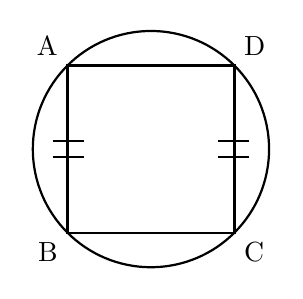
\begin{tikzpicture}[scale=1]

  % Define the center of the circle
  \coordinate (O) at (0,0);

  % Define the radius of the circle
  \def\R{1.5}

  % Draw the circle
  \draw[thick] (O) circle (\R);

  % Define the vertices of the inscribed square
  % The square is inscribed in the circle, so the vertices lie on the circle.
  % We use polar coordinates to define the vertices.
  \coordinate (A) at (135:\R);
  \coordinate (B) at (225:\R);
  \coordinate (C) at (315:\R);
  \coordinate (D) at (45:\R);

  % Draw the square ABCD
  \draw[thick] (A) -- (B) -- (C) -- (D) -- cycle;

  % Add labels for the vertices
  \node[above left] at (A) {A};
  \node[below left] at (B) {B};
  \node[below right] at (C) {C};
  \node[above right] at (D) {D};

  % Double tick marks on side AB
  \draw[thick] (-1.25, 0.1) -- (-0.85, 0.1);
  \draw[thick] (-1.25, -0.1) -- (-0.85, -0.1);

  % Double tick marks on side CD
  \draw[thick] (1.25, 0.1) -- (0.85, 0.1);
  \draw[thick] (1.25, -0.1) -- (0.85, -0.1);

\end{tikzpicture}